\documentclass[a4paper, 11pt]{article}

\voffset -0cm
\hoffset 0.0cm
\textheight 23cm
\textwidth 16cm
\topmargin 0.0cm
\oddsidemargin 0.0cm
\evensidemargin 0.0cm


\usepackage{subfigure}  
\usepackage{setspace}
\usepackage{algorithm2e} 
\usepackage{fancyheadings}
\usepackage{amsmath}
\usepackage{amssymb}
\usepackage{graphicx}
\usepackage{url}
\usepackage{overpic}
\title{}
\author{}
\date{}

\newtheorem{qu}{Question}

\newtheorem{qustar}[qu]{Question $\star$}

\newcommand{\textbox}[1]{\noindent\fbox{
\begin{minipage}{\textwidth}
\usefont{T1}{cmbr}{m}{n} #1  \end{minipage}}}


\begin{document}

\begin{center}
	\LARGE \textbf{``Images et g\'eom\'etrie discr\`ete''\\Final Exam (3h)}
\end{center}


All exercises are independent. All material (lecture notes, slides) are
allowed. Questions with $\star$ symbols may be
more difficult and thus may give you extra points. 



\section{``But for the chicken, where are the ears ?''}
\label{sec:but-chicken-where}

Jesse P. and Walter W. are cookers in Gustavo F.'s restaurant ``Los
Pollos Hermanos''.  They have to prepare a new recipe based on fried
chicken ears. Walter, who is quite skilled in sciences, suggests the
following thing: ``Let's model the chicken as a simple polygon
$P=(v_1,\ldots,v_n)$  (ordered clockwise, no self-intersection, single connected
component) and let's define an \emph{ear} of a polygon at $v_i$ by three
consecutive vertices $(v_{i-1},v_i,v_{i+1})$ such that the  segment
(\emph{chord})
$[v_{i-1}v_{i+1}]$ lies in the interior of $P$'' (since $P$ is simple,
we can always distinguish  interior from exterior).

Jesse: ``Okay... but where are the ears ?''

Walter: ``I'll show you that any polygon has at least two ears''

Jesse: ``Yo great.. Let's cook!''


\begin{qu}
  Let's start by a warm-up: first prove the following statement:
  \begin{center}
    $v$ is an $ear$ of $P$ $\Leftrightarrow$ it's interior angle is
    less than $\pi$ and
    there is no vertex $z$ of $P$ inside the triangle
    $(v_{i-1},v_i,v_{i+1})$.
  \end{center}
\end{qu}


\begin{qu}
  At a given vertex $v$ of $P$, give the pseudo-code of the function
  which returns true if a vertex $z$ belongs to the triangle
  $(v_{i-1},v_i,v_{i+1})$ (false otherwise). Please make sure that you
  use the exact geometrical predicate \texttt{Orientation}$(a,b,c)$.

  Give the pseudo-code of the function which returns true if $v$ is an
  ear of $P$.  What is its complexity ?
\end{qu}


In the following question, we prove the following statement: For any
simple polygon $P$ with at least 4 vertices, $P$ has at least two
\textbf{non-overlapping} ears (non-overlapping is important in
proofs).  The proof will be done by induction on the number of
vertices of $P$. Let's denote by $H(k)$ the hypothesis that the
statement is true for any $P$ with at most $k$ vertices.

\begin{qu}
  First prove that we have $H(4)$.
\end{qu}

We assume that $H(n-1)$ is true and that $P$ has $n$ vertices. We want
to prove $H(n)$.

\begin{qu}
  Let us consider a convex vertex $v$ of $P$ (vertex with
  interior angle less that $\pi$). We call
  $v^-$ (respectively $v^+$) the previous vertex (resp. next vertex)
  of $v$ on $P$.  If $v$ is an ear, prove that $P$ as at least two
  non-overlapping ears.
\end{qu}


\begin{qu}
  If $v$ is not an ear,  there exists a vertex $z$ of $P$ inside the
  triangle $(v^-,v,v^+)$.  Let $L$ be the line parallel to $(v^-,v^+)$
  going through $z$ (if there are several points inside the triangle
  $(v^-,v,v^+)$, $z$ will be such that it gives a line $L$ closest to
  $v$), see Figure \ref{fig:P}.

  Show that the chord $[vz]$ is inside $P$.

  Use this chord to split $P$ and complete the proof.
\end{qu}

\begin{figure}
  \begin{center}
    \subfigure[]{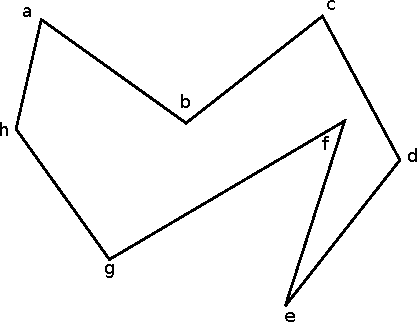
\includegraphics[width=7cm]{ear}}
\subfigure[]{   \begin{overpic}[width=7cm]{P}
      \put(45,-3){$v$}
      \put(46,10){$z$}
      \put(5,25){$v^-$}
      \put(95,18){$v^+$}
      \put(90,6){$L$}      
      \put(27,12){$a$}      
      \put(70,8){$b$}      
    \end{overpic}}
  \end{center}
  \caption{Illustration for Exercise \ref{sec:but-chicken-where}. In
    $(a)$, only vertices $\{a,e,g,h\}$ induce ears.}
  \label{fig:P}
\end{figure}


\begin{qu}
  Show how this property can be used to triangulate any simple
  polygon. What would be the complexity of such process ? How many
  ears Walter and Jesse will get from a polygonal chicken with $n$
  vertices ? Is it a good deal for Gustavo ?
\end{qu}


\textbox{The original proof has been given by G.H. Meisters in
  ``\emph{Polygons Have Ears}'', The American Mathematical Monthly,
  82(6):648--651, 1975. The questions follows Meisters's workflow.}

\section{CarWash}

Skyler W. is running a car-wash business and she wants  to set-up a
license plate recognition system in a do-it-yourself mode. Walter
W. (her husband) has suggested her to consider mathematical morphology
tools for that.

Let us first recall some definitions from the lecture on mathematical
morphology on a set $E$:
\begin{itemize}
\item $A,B,X$ are subsets of $E$;
\item $B_x$ with $x\in E$ is $\{ z+x \,|\, z\in B\}$ (translation of
  $B$ from $x$);
\item Dilation of $X$ by a structuring element $B$:
  \begin{displaymath}
    \delta_B(X) =  X \oplus B = \bigcup_{x\in X} B_x =
    \bigcup_{b\in B} X_b\,;
  \end{displaymath}
\item Erosion of $X$ by a structuring element $B$:
  \begin{displaymath}
   \epsilon_B(X) = X \ominus B = \{z\in E | B_{z} \subseteq
    X\} = \bigcap_{b\in B} X_{-b}\,;
  \end{displaymath}
\item Opening: $A \circ B = (A \ominus B)\oplus B$;
\item Closing: $A \bullet B = (A \oplus B)\ominus B$.
\end{itemize}

For grayscale/scalar images, the erosion and dilation are given as follows:
\begin{align*}
  (F\oplus G)(x) = \sup_{y\in E} \{ F(y) + G(x-y)\}\,,\\
  (F\ominus G)(x) = \inf_{y\in E} \{ F(y) - G(x-y)\}\,.
\end{align*}


\begin{qu}
  Consider the following set $X\subset\mathbb{R}^2$ given by black unit
  squares (left).
    \begin{center}
    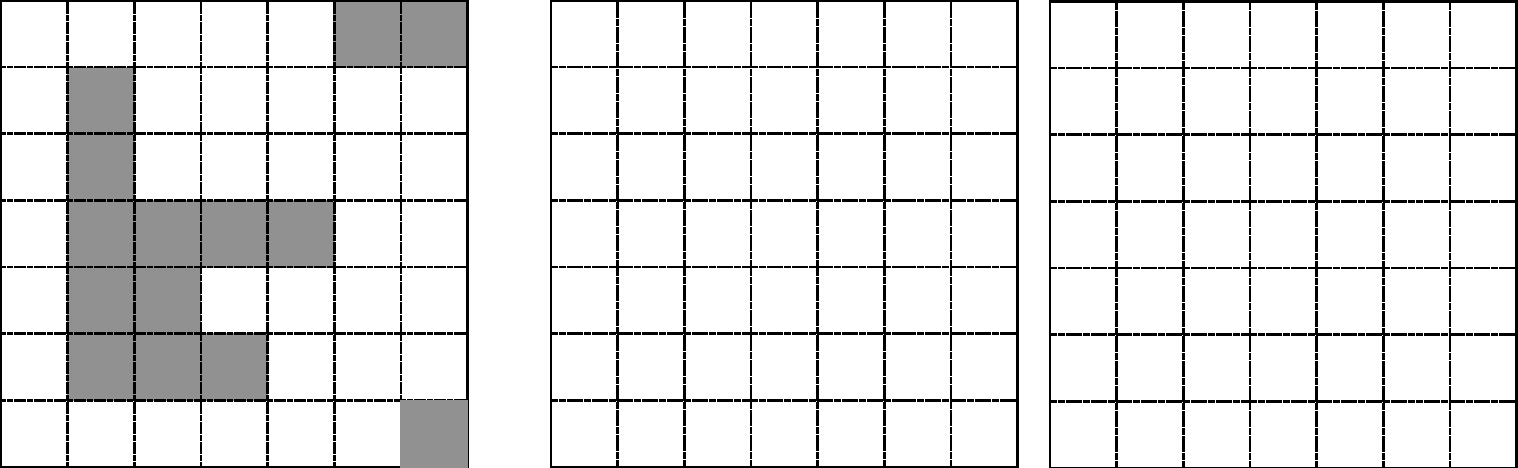
\includegraphics[width=12cm]{morpho1}
    \end{center}
    Could you please draw  the result of the dilation (middle)
   and the result of the erosion  (right) of $X$ by a structuring
   element $B$ which is an open Euclidean disk with radius 1.

\end{qu}

\begin{qu}
  Let us consider this simple structuring element on scalar functions:
  \begin{center}
    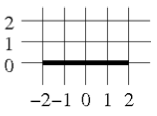
\includegraphics[width=3cm]{elemstruct}
  \end{center}
We consider a simple 1D grayscale image as depicted below (please,
only consider the discrete values only). Using the above mentioned
structuring element, use the empty grids to draw
the result of the erosion and dilation operators of this 1D image.
 \begin{center}
    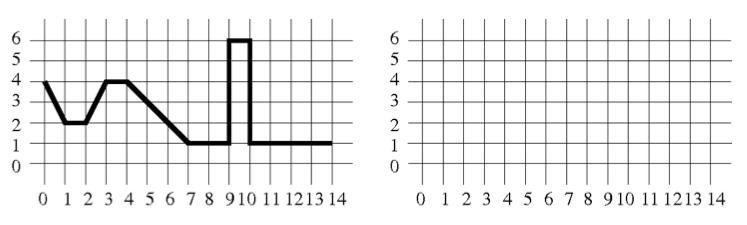
\includegraphics[width=14cm]{1d}
    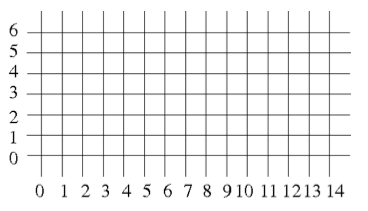
\includegraphics[width=7cm]{grille1d}
    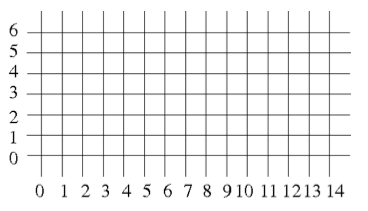
\includegraphics[width=7cm]{grille1d}
  \end{center}
\end{qu}



\begin{qu}
  Skyler have tested some preliminary operators (see
  Fig~\ref{fig:license}). On the input image
  Fig~\ref{fig:license}$-(a)$, she got the two images
  Fig~\ref{fig:license}$-(b)$ and  Fig~\ref{fig:license}$-(c)$. What
  morphological operators did she use ? Why has she considered  them ?
\end{qu}


\begin{figure}[!htbp]
  \begin{center}
    \subfigure[]{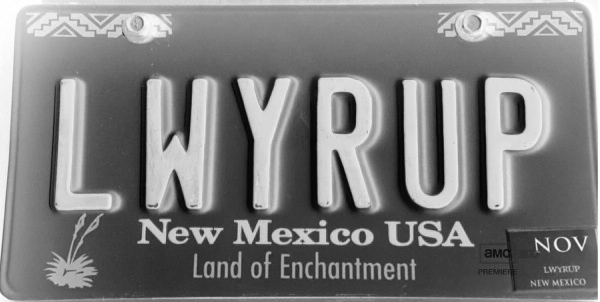
\includegraphics[width=8cm]{saul}}\\
    \subfigure[]{
\includegraphics[width=7cm]{saul-vert}}
    \subfigure[]{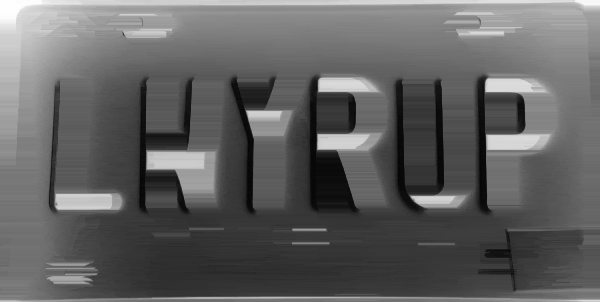
\includegraphics[width=7cm]{saul-horiz}}
  \end{center}
  \caption{License plate example: $(a)$ Skyler's input and $(b)-(c)$ her results.}
  \label{fig:license}
\end{figure}


\section{Pinkman's Theorem}


Before breaking bad as a cooker in Gus's restaurant, Jesse was a nice
college student. In fact, he proved a great result on lattice polygon, the Pinkman's
theorem. Actually, several typos later, this result is now known as
\emph{Pick's theorem} (very  famous  in digital geometry).

For short, given a simple polygon $P$ with integer coordinate
vertices (lattice polygon), this theorem links the (Euclidean) area of $P$
$\mathcal{A}(P)$ with its number of (digital) interior points $I_P$
and the number of (digital) points on its boundary $B_P$:
\begin{equation}
\label{eq:pinkmans-theorem}
  \mathcal{A}(P) = I_P + \frac{B_P}{2} - 1 
\end{equation}

\begin{figure}
  \begin{center}
    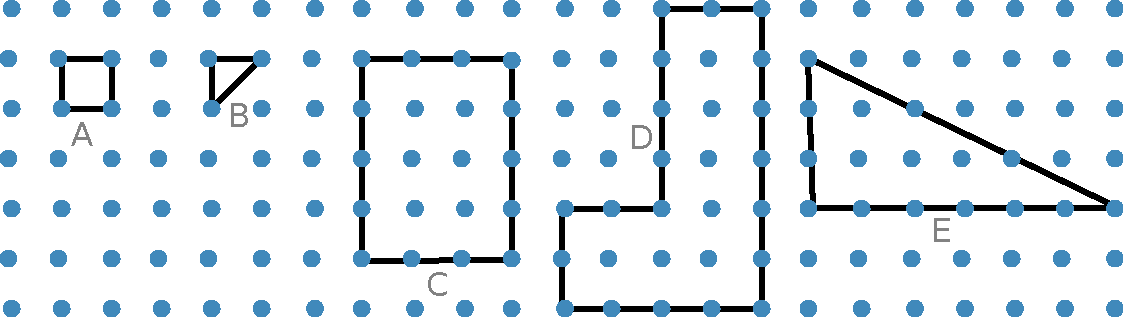
\includegraphics[width=14cm]{pick}
  \end{center}
  \caption{Examples for Pinkman's theorem.}
  \label{fig:pick}
\end{figure}
\begin{qu}
  For shapes depicted in Figure \ref{fig:pick}, give the
  $\mathcal{A}$, $I$ and $B$ quantities and show that
  Eq.~(\ref{eq:pinkmans-theorem}) is true for these lattice polygons.
\end{qu}



To prove this theorem, let us first consider elementary shapes:

\begin{qu}
\label{quQuad}
  For a rectangle with width $m$ and height $n$ (in
  Fig.~\ref{fig:pick}, we have $m=3$ and $n=4$ for the rectangle), prove
  that the result holds.
\end{qu}


\begin{qu}
  Consider now a \emph{axis-aligned} right triangle $T$ (rightmost shape in
  Fig.~\ref{fig:pick}), prove the theorem for this object.

  {Hint: use the result of previous question with a variable $k$ which
    is the --unknown-- number of digital points on the triangle
    diagonal}
\end{qu}


To get the final result, we need a last ingredient: the general
triangle.

\begin{qu}
  Using previous results (or assuming that the theorem is true for
  rectangles and axis-aligned right triangles), prove that the result also holds for
   triangles with interior angles less than $\frac{pi}{2}$.

  {Hint: consider the bounding box of the triangle and decompose
    it into $T$ and three right triangles.}
\end{qu}

If one of the triangle angle is greater than $\frac{pi}{2}$, we assume
that Eq.~(\ref{eq:pinkmans-theorem}) is true.

\begin{qu}
  Consider now two lattice polygons $P_1$ and $P_2$, we assume that
  $P$ is given by gluing together $P_1$ and $P_2$ along an edge $e$ (the edge
  $e$ belongs to both lattice polygon $P_1$ and $P_2$).

  If Eq.~(\ref{eq:pinkmans-theorem}) is true for both $P_1$ and $P_2$,
  prove that this result is also true for $P$.

  Hint: consider the number of points on $e$.
\end{qu}



\begin{qu}
  Using the results of Exercise~\ref{sec:but-chicken-where}, can you
  conclude to prove the theorem for general simple lattice polygon ?
\end{qu}


Now, let's play a bit with arithmetic of lattice polygons (again, all
points and vectors have integer coordinates).

\begin{qu}
  For a straight segment $[(0,0) - (u,v)]$ what are the properties on
  $u$ and $v$ to have only two digital points on it, the extremities ?
\end{qu}


\begin{qu}
  Let $P$ be a parallelogram defined by the two vectors $(37,7)^T$ and
  $(9,2)^T$ and origin point $(0,0)$. How many boundary points have $P$
  ? How many interior points ? 
\end{qu}

\begin{qu}
  Applying Eq.~(\ref{eq:pinkmans-theorem}), what is the area of the
  parallelogram defined by $(37,7)^T$ and $(9,2)^T$ ?
\end{qu}
and more generally:
\begin{qu}
\label{questionuv}
  For two vectors $(u,v)^T$ and $(w,t)^T$, what are the properties on
  $u,v,w$ and $t$ so that there is no interior point in the
  parallelogram defined by these vectors and $(0,0)$ ?
\end{qu}



\begin{qustar}
  Let's apply the following transformation to each vertex
  $(i,j)\in\mathbb{Z}^2$ of a lattice polygon $P$:
  \begin{equation}
    (x,y) = \left (
    \begin{array}{cc}
      u & w\\
      v &t
    \end{array}\right)\cdot \left ( 
    \begin{array}{c}
      i\\j
    \end{array}\right)
  \end{equation}
using $u,v,w,t$ has described in Question~\ref{questionuv}. Let $P'$
by the resulting polygon from the transformation of $P$ vertices. Is
the obtained polygon $P'$ still a lattice polygon ? What is its area
and number of boundary points ?
\end{qustar}



\begin{qustar}
  If we suppose that the lattice polygon has $n$ holes (each hole boundary
  being defined by a simple lattice polygon), a similar result for
  Eq.~(\ref{eq:pinkmans-theorem}) exists. Can you guess the general
  formula ? (Hints: draw some examples with 1, 2 and 3 holes...)
\end{qustar}


\textbox{Let's be honest, Jesse was not really interested in
  mathematics, original result is due to Georg Alexander Pick in
  1899.}


\end{document}

